\documentclass[article]{elsarticle}
%\documentclass[draft]{elsarticle}

\usepackage{lineno,hyperref}
\modulolinenumbers[5]

%\usepackage[english]{babel}
%\usepackage[utf8x]{inputenc}
%\usepackage[T1]{fontenc}
%

\usepackage{threeparttable}
\usepackage{graphicx}
\usepackage{subfig}
\usepackage{setspace}
%% potrzebne do tabeli jak w przykładzie
\usepackage{tabularx}
\newcolumntype{C}{>{\centering\arraybackslash}X}
%
\usepackage{epstopdf}
\usepackage{amssymb}
\usepackage{gensymb}
\usepackage{amsmath}
\usepackage{tabularx}
\usepackage{multirow}
\usepackage{float}
\usepackage{polski}
\usepackage[utf8]{inputenc}
\restylefloat{table}
%%\usepackage{multirow}
\usepackage{booktabs}
%\usepackage{authblk}
\usepackage[bottom]{footmisc}
\usepackage[figurename=Fig.]{caption}
\usepackage[section]{placeins}
\usepackage{color, soul} % highlighting
\newcolumntype{Y}{>{\centering\arraybackslash}X} %necessary for tabularx to make equal width columns
\usepackage[usenames,dvipsnames]{xcolor} 
\usepackage[draft]{todonotes}   % notes showed; should be after xcolor

\usepackage{makecell}

\newcommand{\hlc}[2][yellow]{ {\sethlcolor{#1} \hl{#2}} }



\journal{Applied Energy}



%%%%%%%%%%%%%%%%%%%%%%%
%% Elsevier bibliography styles
%%%%%%%%%%%%%%%%%%%%%%%
%% To change the style, put a % in front of the second line of the current style and
%% remove the % from the second line of the style you would like to use.
%%%%%%%%%%%%%%%%%%%%%%%

%% Numbered
%\bibliographystyle{model1-num-names}

%% Numbered without titles
%\bibliographystyle{model1a-num-names}

%% Harvard
%\bibliographystyle{model2-names.bst}\biboptions{authoryear}

%% Vancouver numbered
%\usepackage{numcompress}\bibliographystyle{model3-num-names}

%% Vancouver name/year
%\usepackage{numcompress}\bibliographystyle{model4-names}\biboptions{authoryear}

%% APA style
%\bibliographystyle{model5-names}\biboptions{authoryear}

%% AMA style
%\usepackage{numcompress}\bibliographystyle{model6-num-names}

%% `Elsevier LaTeX' style
\bibliographystyle{elsarticle-num}
%%%%%%%%%%%%%%%%%%%%%%%

\begin{document}

\begin{frontmatter}

\title{...}
 
 \author[pwr]{first}
 
 \author[pwr]{second}
   
 \author[pwr]{S\l awomir Pietrowicz\corref{cor1}}
 \ead{slawomir.pietrowicz@pwr.edu.pl}
 
 \cortext[cor1]{Corresponding author Tel.: +48 71 320 36 17}
 
 \address[pwr]{Department of Thermodynamics, Theory of Machines and Thermal Systems, Faculty of Mechanical and Power Engineering, Wrocław University of Technology, Wrocław Wybrzeże Wyspiańskiego 27, Poland}


\begin{abstract}

\end{abstract}

\begin{keyword}
\hlc{Oscillating} Heat Pipe \sep  \sep  \sep 
\end{keyword}

\end{frontmatter}

\linenumbers

\section*{Nomenclature}

\begin{tabular}{l c p{10.5cm}}

  $A_c$ & -- & cross-sectional area of the tube, $\mathrm{m^2}$ \\
  $I$ & -- & input current, $\mathrm{A}$ \\
  $U$ & -- & input voltage, $\mathrm{V}$ \\
  $T$ & -- & temperature, $\mathrm{K}$ \\
  $\bar{T}$ & -- & average temperature, $\mathrm{K}$ \\
  $R$ & -- & thermal resistance, $\mathrm{K/W}$ \\
  $P$ & -- & pressure, $\mathrm{Pa}$ \\
  $Q$ & -- & heat load, $\mathrm{W}$ \\
  $\dot{Q}$ & -- & heat flux, $\mathrm{W/m^2}$ \\
  $t$ & -- & time, $\mathrm{s}$ \\  
\end{tabular} 
\\ 

\textit{ Greek symbols}

\begin{tabular}{l c p{10.5cm}}

  $\rho$ & -- & density, $\mathrm{kg/m^3}$ \\
  $\sigma$ & -- & ..., $\mathrm{N/m}$ \\
       
\end{tabular} 
\\ 
%\textit{ Superscripts}

\textit{ Subscripts}

\begin{tabular}{l c p{10.5cm}}
 
  $l$ & -- & liquid \\
  $v$ & -- & vapor \\
  $h$ & -- & heating \\
  $c$ & -- & condenser section \\
  $e$ & -- & evaporator section \\
  $m$ & -- & mean value \\
  $crit$ & -- & critical value \\     
\end{tabular} 
\\

\textit{Abbreviations}

\begin{tabular}{l c p{10.5cm}}

  $PHP$ & -- & Pulsating Heat Pipe \\  
       
\end{tabular} 

\section{Introduction}
\label{sec:intro}
Conventional heat removal systems in industrial installations generally require the supply of external energy. The widespread tendency of process optimization (due to technological development) and reduction of their energy consumption place all technologies of passive heat transport in the center of attention. Pulsating heat pipes not only as simple structure devices, but also with excellent heat transfer capabilities are passive exchangers, which allows them a wide range of applications in industrial processes.\\
The heat transfer characteristics in PHP are complex due to the associated two-phase flow phenomena. It has been shown by previous researchers that the operating conditions of the device are regulated by many factors such as tube material[A,I,J], the number of turns[F], inner diameter[k,O], type of working fluid[B,C,P],  its filling ratio[D,P,U], the inclination angle influece [W,V] and meany others for example as mentioned in [E].\\ 
One of the most influential factors on device performance is the working fluid. It is its filling ratio and thermo-physical properties, such as specific heat, latent heat of evaporation, density or boiling point, determine the efficiency and operating conditions of the entire device. The lower the fluid latent heat of evaporation, its the lower operating temperature of the start-up condition, but also its the greater susceptibility to the occurance of the dry-out phenomenon [T]. With respect to the medium not only pure fluids as in [L] works, but mixtures of various fluids [N,R,S] and also  with additions of solid particles (nanofluids) as [H,M], are used. The amount of working fluid in the circuit has a direct impact on the exchanger operating conditions, its low amount is the low friction factor between the fluid and wall interface, which increases the flow. At the same time, a small volume of liquid inside of the system means a lot of free space for the steam which results in a tendency to faster dry-out. On the other hand, the greater amount of the working fluid causes a higher pressure required to generate motion between the heating/cooling sections, higher friction forces, but also higher values of transmitted sensible heat. To sum up any influence of the quantity or properties of the working medium, literature mostly declares the optimal its amount as 50$\%$ [X, W].\\
The efficiency of the pulsating heat pipe depends on the material it is made of. [A] presents fabrication and experimental evaluation of a polymer-based flexible pulsating heat pipe. The authors show unusual flexibility in the use of passive heat removal technique using PHP. Not enough that it can be made of plastic, in addition, the construction of its flow channel can have an advanced geometry at the same time allowing for easy assembly thanks to its flexible construction. In conclusion, all together reduces the overall thermal resistance of the device by 37$\%$ compared to a tube made of copper.\\
It has been confirmed that the effect of the device's energy efficiency is also determined by the stable direction of the flow inside the exchanger called as a self-sustained circulatory motion. The work [XXX] presents a system with a check valve, which forces fluid movement inside the tube in only one direction. In effect it reduces the thermal resistance of PHP by 25$\%$ compared to set without check valve. In the publication [XXXX], a directional flow was obtained thanks to the ball valve, which resulted in a 10-14$\%$ higher heat transport capacity. Flow directionality can be obtained also in another way, i.e. at work [MARCO MARENGO!]. After applying an asymmetrical heating system (heating only on the left or right side and in the center), a specific direction of the working fluid movement was forced, which translated into a reduction in the thermal resistance of ... on ....\\
From a number of geometric parameters affecting on PHP performance, most are already well researched. Only the variable length of the adiabatic section compared to the amount of the working fluid or its type does not appear too often in the publications. In order to properly optimize the occurring thermal-flow processes during the heat transport, knowledge of the influence of the distance between heating and cooling sections on the efficiency of the exchanger is required. A. D. Fonseca et al. [G] conducted research on thermal performance of a cryogenic helium pultasing heat pipe.The authors comparing the two lengths, i.e. 0.3 and 1m adiabatic section, provided conclusion that the regime in which the exchanger operates does not change (the temperature of the diffrence between the evaporator and condenser section)in compared cases. Also maximum thermal conductivity for the PHP with 1m lenght of adiabatic section, compared to 0.3m, was aproxymatley three times higher. Literature review indicates that most of the tests carried out on pulsating heat pipes contain experimental studies with the conclusion on thermal efficiency, which can reach up to 300 kW / mK [Y] in cryogenic applications for heat pipes.\\
This paper presents the built test stand of a pulsating heat pipe in a stationary system for incremental heat inputs in evaporation section with variable filling ratio and adiabatic section length compared to the three different fluids. The thermal resistances and performances values have been compared for each solution to determine the influence of variable parameters on the thermal and flow processes taking place inside the device.


\section{Experimental setup}
\subsection{Working fluid selection}

Thermo-physical properties of the working fluid have a direct impact on PHP's heat transfer performance. In order to well understand the involved processes and their appropriate analysis, three factors were selected, i.e. acetone, ethanol and deionized water as shown in Tab.\ref{table:properties}.

\begin{table}[H]
\caption{Thermodynamic properties of acetone, ethanol and water at $20^0C$.}
	\centering
	\begin{tabular}{lcccc}
	\hline
		Properties & Acetone& Ethanol & DI Water\\
	\hline
		Boiling point, $^oC$ & $56.2\cdot$& $78.3$ & $100\cdot\cdot$\\
        Saturation pressure, kPa & $24.66\cdot\cdot$ & $5.88$ & $2.34\cdot$\\
		Latent heat of vaporization, kJ/kg & $523\cdot$ & $846$ & $2257\cdot\cdot$\\
		Liquid density, $kg/m^{3}$ & $792\cdot$ & $789\cdot$ & $998\cdot\cdot$\\
		Dynamic viscosity, $Pa\cdot s$ & $0.32\cdot$ & $1.15\cdot\cdot$ & $1.01$\\
        Surface tension, $N/m$ & $23.7\cdot$ & $22.8\cdot$ & $72.8\cdot\cdot$\\
        Critical tube diameter$^*$, mm & $3.47\cdot$ & $3.40\cdot$ & $5.45\cdot\cdot$\\
        Liquid specific heat, $kJ/kgK$ & $2.35\cdot$ & $2.39\cdot$ & $4.18\cdot\cdot$\\
        Thermal conductivity, $W/mK$ & $0.170\cdot$ & $0.172\cdot$ & $0.599\cdot\cdot$\\
	\hline
	\end{tabular}
    	\begin{tablenotes}
		\item[\textdagger]\small{Highest were marked by two dots and the near lowest/lowest was marked by dot \\ * calculated from Eq.\ref{Eqn:d_crit} with reference value from CoolProp}
	\end{tablenotes}
	\label{table:properties}
\end{table}
\subsection{PHP preparation} 
The construction of PHP fig.\ref{jdm1} contained $14$ meandering bends, with the possibility of reducing them to $2$. During the heat exchange process inside of the capillaries complicated processes occur, resulting in a multiphase flow of the working fluid. It has been proven that the flow structures depend on the operating conditions of the exchanger, therefore, in order to be able to take into account these changes during the tests, the heat pipe was built of two materials. The first was toughened laboratory glass, borosilicate, with the total lenght of $0.5$, $0.75$ and $1m$, used on straight parts of exchanger, for flow visualization and partial implementation the function of the adiabatic (quasi-adiabatic) section. The second one was copper, which was the material used to build the condenser/evaporator u-shapes (bending radius $R=35mm$) to increase heat transfer efficiency and the ability to proper investigation of the process dynamics. It was important to consider the system's response to changes in the heating energy supplied Tab.\ref{table:heatInputs}.\\
\begin{figure}[H]
\centering
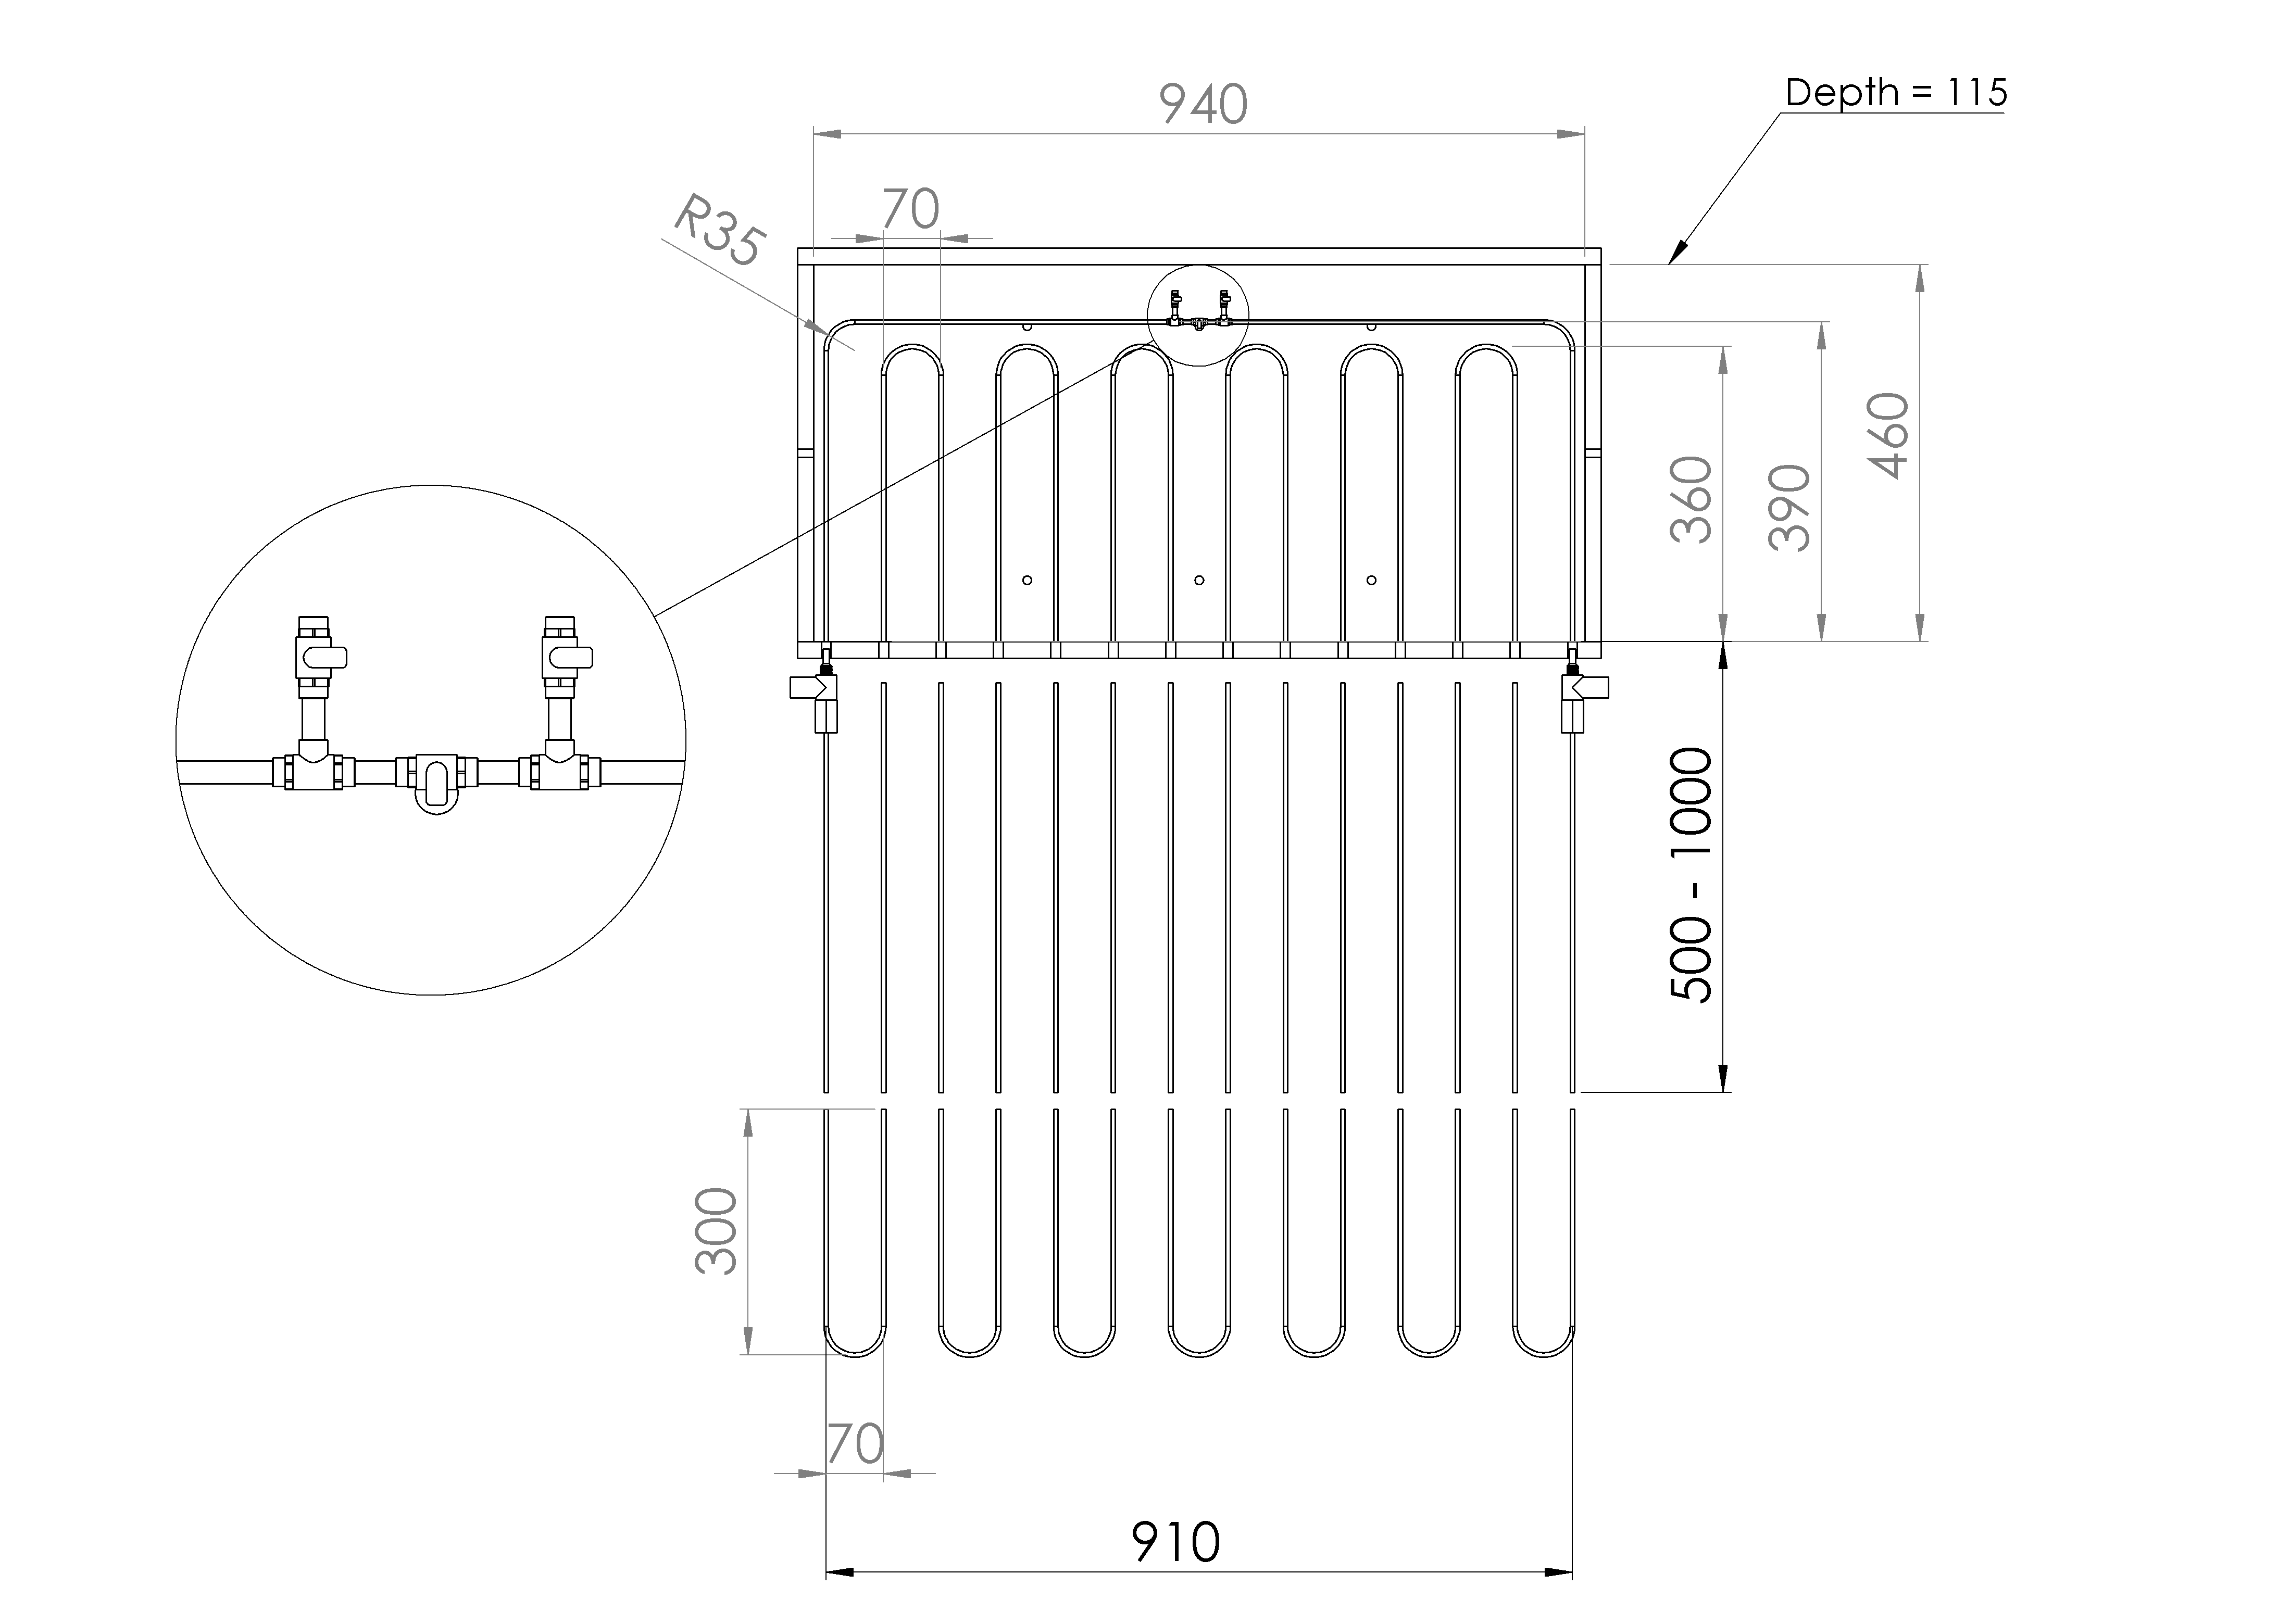
\includegraphics[width=1\textwidth]{figures/Wizualizacja.png}
\caption{\hlc{Basic dimensions of experimental setup}}
\label{jdm1}
\end{figure}

\begin{table}[H]
	\centering
	\caption{The geometrical configuration of heat eschanger}
	\begin{tabular}{lcccc}
	\hline
		Condenser length & $$ & $$ & $..$\\
		Evaporator length & $$ & $$ & $..$\\
		PHP length & $$ & $$ & $.. .. ..$\\
		Adiabatic length & $$ & $$ & $500$, $750$ and $1000$mm\\
        Filling ratio & $$ & $$ & $25$, $50$ and $75$\%\\
        Inner diameter & $$ & $$ & $2.5$mm\\
        Number of turns & $$ & $$ & $14$\\
        ... & $$ & $$ & $...$\\
        ... & $$ & $$ & $...$\\
	\hline
	\end{tabular}
	\label{table:configuration}
\end{table}

The cooling task was carried out by a device system connected to the condenser section by means of a $42L$ cubic tank. In order to increase the intensity of heat removal and also due to the considerable length of the exchanger, the inlets/outlets of the cooling water to and from the tank were doubled. The inlets were placed on the left and right side of the housing and the water was removed from two points located in the middle of the PHP length. The tank was made of six $0.1mm$ thick tarnamid plates, which allowed to obtain a satisfactory isolation from the ambient conditions. The heating plate has been subjected to an appropriate treatment, computer-controlled, to create for copper pipes passable thermal grease with heating plate surface and channels for thermocouples to prevent them from being cut after folding the heating section together. Whole thermal block (heaters and heating plates) was well insulated by glass woll and closed in metal housing.\newline
\indent The quasi-adiabatic and heating/cooling sections were combined by the especially designed and made for the project only, glands which was sealed on the glass using a set of O-rings and beveled washers. On the other side, the glands sealed the copper u-shapes using clamping barrels mounted on sleeves (used to determine one external dimension for all metal elements of the exchanger). The seals were chosen to be to aggressive fluids and high temperature resistant. By using this solution, it was possible to change the working fluid, the diameter of the flow channel and the length of the quasi-adiabatic section, because the glass was produced with a constant external diameter but variable the internal. The last element, and the second construction unit in this setup, was the support frame with its own drive and inclinometer, which allowed for a free change in the inclination angle of the exchanger in the range of $0\div90$ degree. It should be noted that in this study the vertical, bottom heat mode was employed.



\subsection{Experimental apparatus}
Experimental setup due to complex thermal-flow processes and the introduced geometric changes of exchanger required the equipment of control and measurement instruments. Condenser temperature was kept at \hlc{288}K by isothermal cold bath circulator (volumetric flow rate to $20$ $l/min$) with $\pm0.5K$accuracy. In order to investigate the effect of various heat loads supplied to the evaporator section, the DC power supply with a power range of $0\div2000W$ ($6675A$, Agilent Technologies, USA) were used. The device was equipped with an analog control of voltage ($0\div120V$) and current ($0-16A$) output with the possibility of control via the GPIB port. All temperature measuring points located as shown (\hlc{odniesienie do rysunku z termoparami}) are equipped with T-type thermocouple wires of diameter of $0.1mm$ with accuracy $0.5K$. The temperature was mesured on the external wall of heaters and capillaries by soldering, glass surface by gluing and cooling water inlet / outlet through chokes in supply pipes (thermocouple tips located in the middle of the cross-secional flow). Piezoresistive absolute pressure transmitter ($S-20$, WIKA Instrument Lp, Poland) with heat sink was installed close to the condenser on the quasi-adiabatic section by a measuring nozzle, appropriately designed and manufactured for the project, having as little impact on the disturbance of the flow channel as possible, while measuring the pressure fluctuation inside the pipes. The PHP was evacuated for underpressure of \hlc{...}Pa with an oil-free rotary vacuum pump (nXDS10i, EDWARDS LC, UK). The current volumetric flow rate of cold water was measured using a flow meter (Flowmax $44i$) based on the ultrasonic technology with no moving parts able to measure conductive and non-conductive liquids. The device has been calibrated to provide accuracy of less than $0.3 l/min$.\\
All signals as pressure, temperature, volumetric flow of cold water and power supply could have beed acquired. High speed data aqusition system based on National Instruments brand components in combination with a \hlc{computing station} gave the opportunity to perform control and measurement of setup together with data recording and processing.
\subsection{Test conditions and procedure.}
Due to separable connections between the sections of the exchanger, without any kind of adhesives or sealants, the system before each series of measurements had to be leak tested. In the first place, a vacuum of $4\cdot 10^3 mbar$ was produced with an oil-free vacuum pump, which enabled the turbomolecular pump to be activated, causing the flow from the exchanger through the spectrometric analyzer. Then, using helium, it was checked whether the exchanger had leaks. After performing the appropriate tests for the given adiabatic section length, all o-ring packages were exchanged for new ones.\newline 
\indent The test procedure provided an analysis of the filling ratio influence on exchanger thermal efficiency. For this reason, every series of measurements regarding the chosen factor was done equally. First, a vacuum was created inside the capillaries to remove non-condensable gases. Then, the volume of $25\%$ of the exchanger was filled with liquid. After performing the appropriate set of measurements, the system was terminated, and after the break of one day, PHP was filled with another portion of the factor of $25\%$ of the total exchanger volume. The operation was repeated so that in the last set of measurements, the heat exchanger filled in $75\%$ examine was provided. Data acquisition in connection with the daytime system cooling down allowed for precise control of the exchanger's leaks. Each time before proceeding to the next measurement day, the stored pressure inside the exchanger before heating and after cooling down was checked. In the case of a difference between these two values, the tests were repeated, after dismantling and reassembling parts of the exchanger.\newline
\indent All measurement sets were performed in accordance with the checklist, which simultaneously implemented the start-up procedure:
\begin{itemize}
\item Air-evacuation from the exchanger until the desired vacuum level is reached.Then, using a set of valves, perform the required filling with an appropriate working fluid.
\item \hlc{Inception} of the cooling process by switching on the aggregate, adjusting the set point temperature and flow of the medium, moving to the next operation after the process has been established.
\item Launching a data acquisition system and equipment supplies. Launching an application which implements the power supply control program, and then start observing the flow structure through the glass capillaries along with data recording through the computer.
\end{itemize}
\indent The most important control parameter was heat provided to the evaporator section. During the experiment a few heat input levels were defined in range between $500 W - 2000 W$ in corresponding time of $10$ hours. The starting heat input was kept at constant level for 2 hours \hlc{while following} were kept at constant level for 1 hour. The list of heat inputs levels with corresponding times and heat fluxes is shown in Table  \ref{table:heatInputs}.

\begin{table}[H]
	\centering
	\caption{Heat input levels provided to the evaporator section}
	\begin{tabular}{lcccc}
	\hline
		\thead{Time,\\ h} & \thead{Heat Input,\\ W} & \thead{Heat flux ($d=2.5 mm$),\\ $kW/m^2$}\\
	\hline
		$0h - 2h$ & $500 W$ & $14.0$\\
		$2h - 3h$ & $750 W$ & $21.0$\\
		$3h - 4h$ & $1000 W$ & $28.0$\\
		$4h - 5h$ & $1250 W$ & $35.0$\\
        $5h - 6h$ & $1500 W$ & $42.0$\\
        $6h - 7h$ & $1625 W$ & $45.5$\\
        $7h - 8h$ & $1750 W$ & $49.0$\\
        $8h - 9h$ & $1875 W$ & $52.5$\\
        $9h - 10h$ & $2000 W$ & $56.0$\\
	\hline
	\end{tabular}
	\label{table:heatInputs}
\end{table}

\subsection{Dokładność-Agnieszka}

Collected data from experiment is temperature of evaporator and condenser section, pressure measured in upper part of adiabatic section, heat input in evaporator section is measured in form of voltage and current. Electric power is dissipated as heat input in evaporator section of PHP. Also in condenser section heat is dissipated using water with volumetric flow $18 l/min$ which provides constant temperature in condenser section $15 \degree C \pm 1 \degree C$. Thermal performance of PHPs can be defined by the thermal resistance which is defined as:

\begin{equation}
D_{crit}=2\cdot\sqrt{\frac{\sigma}{g\cdot(\rho_{l}-\rho_{v})}}
\label{Eqn:d_crit}
\end{equation}

\begin{equation}
R=\frac{T_e-T_c}{\dot{Q}}
\end{equation}

As mentioned heat input is provided using electric power which is controlled via National Instruments hardware and can be calculated using formula:
\begin{equation}
\dot{Q}=U\cdot I
\end{equation}

Zasilacz\\
Programming Accuracy \\
Voltage 0.04+ 120 mV\\
Current 0.1+ 12 mA\\\\

Przeplywomierz\\
Kalibrajca 8punktowa -dokladnosc $1.5\%$\\

When experiment is conducted it is important to estimate total error in all measurements. In this paper thermal resistance, heat transfer coefficient and input power are parameters which need calculating total error. Heat transfer coefficient formula is defined as follows:
\begin{equation}
h=\frac{\dot{Q}}{A\cdot \Delta T}
\end{equation}

\section{Results and discussion}

\begin{figure}[h]
\centering
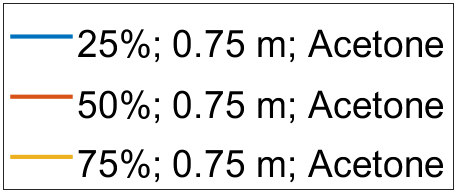
\includegraphics[width=0.4\textwidth]{figures/legend.png}
\caption{\hlc{Sample of chart legend}}
\label{jdm1}
\end{figure}

\begin{figure}[h]
\centering
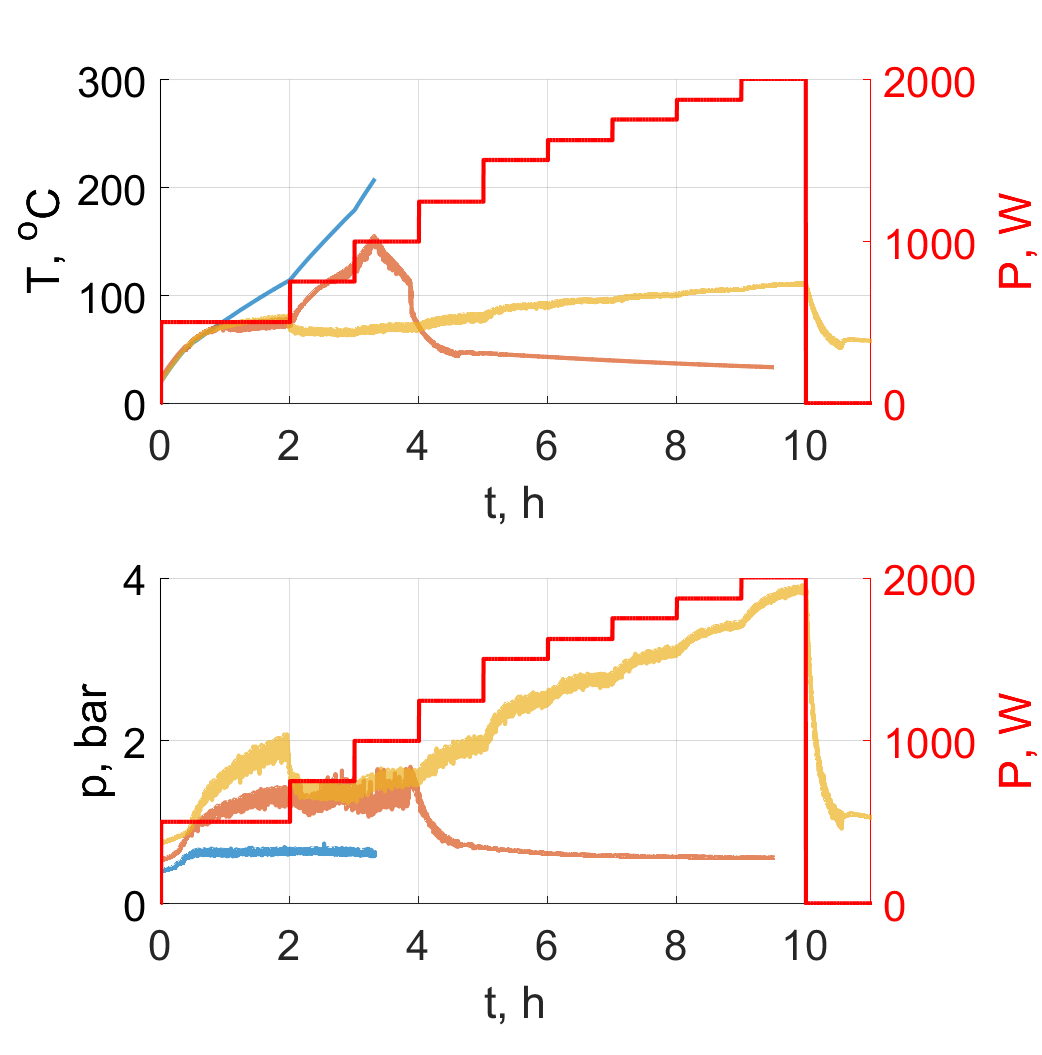
\includegraphics[width=1\textwidth]{figures/Aceton75cm.png}
\caption{Acetone 75 cm, different filling ratios}
\label{jdm1}
\end{figure}

\begin{figure}[h]
\centering
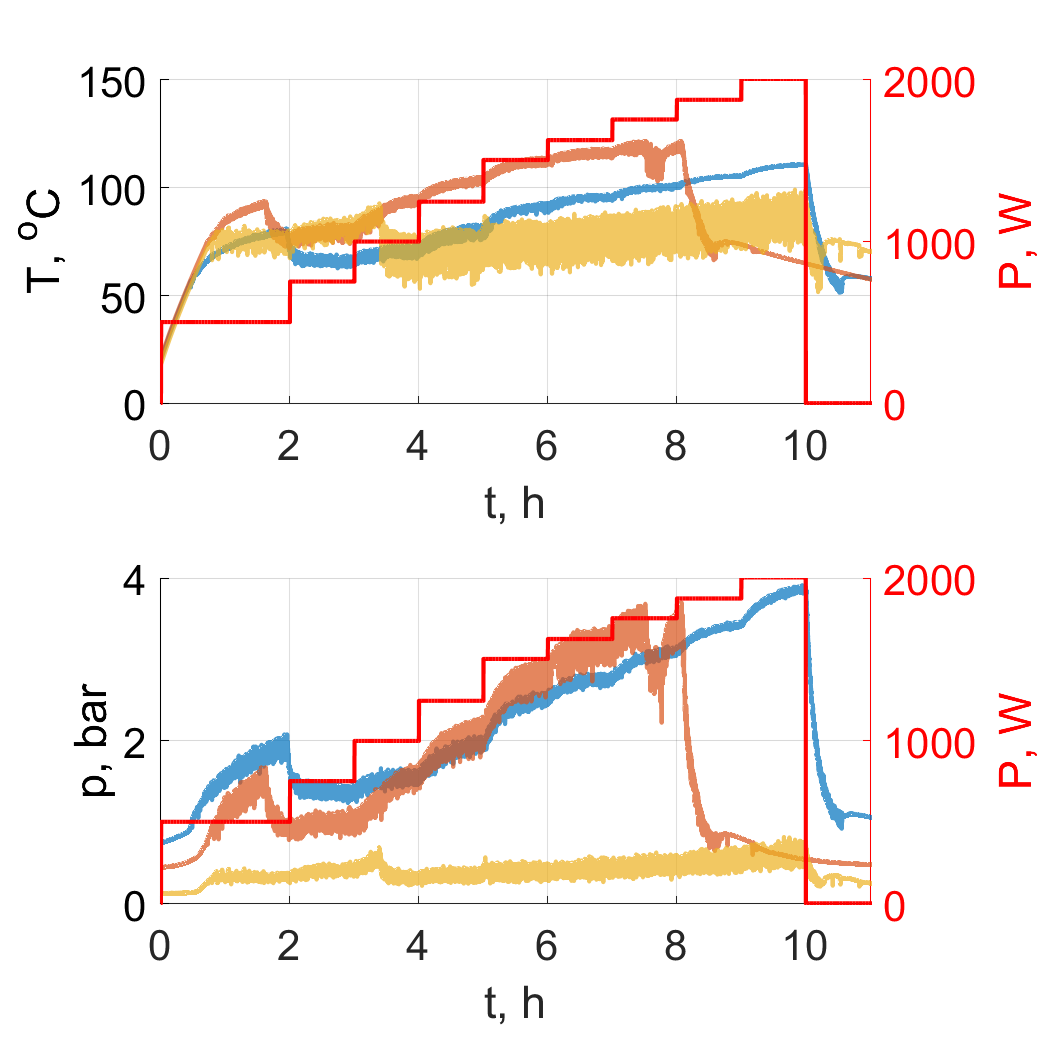
\includegraphics[width=1\textwidth]{figures/AcetonEtanolWoda75cm_1.png}
\caption{75 cm \& 75\%, different working fluids}
\label{jdm1}
\end{figure}

\begin{figure}[h]
\centering
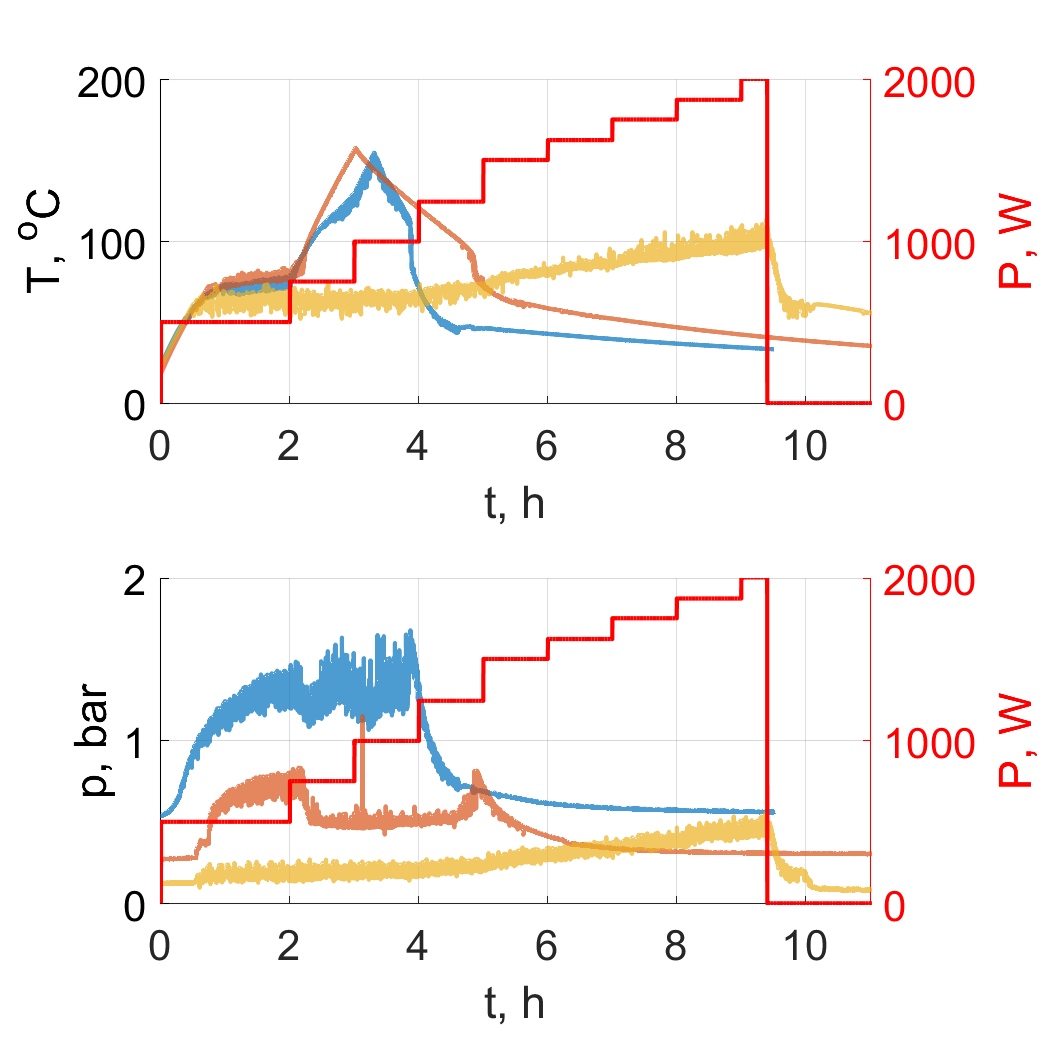
\includegraphics[width=1\textwidth]{figures/AcetonEtanolWoda75cm_2.png}
\caption{75 cm \& 50\%, different working fluids}
\label{jdm1}
\end{figure}


\label{sec:resdis}
\section{Conclusions}
\section*{Conflict of interest}
The authors declared that there is no conflict of interest. 
\section*{Acknowledgements}
The work was financed by Grant No.POiR.04.01.04-00-0037/15. Calculations have been carried out using resources provided by Wroclaw Centre for Networking and Supercomputing (http://wcss.pl).

\section*{References} 

\bibliography{Experimental_PHP.bib}

\end{document}
